\chapter{Expérimentation réalisée et données disponibles} 

\lettrine{C}{e} chapitre explique l'expérimentation qui a été mené en 2017 sur deux vergers dans la commune de Saint-Paul (à la Réunion). 
On reviendra sur le dispositif de l'expérience et les données qui en ont étés tirées.
Le but de cette expérience était de déterminer quel est l'impact de la modalité de couverture du sol dans le degré d'infestation d'un verger.


\section{Dispositif}

Le verger expérimental (que l'on apellera aussi parcelle par la suite) est séparé en trois parts égales de trente arbres.
Sur chacune des trois sous-parcelle, une modalité de couverture du sol différente est mise en place.
Sur un côté il y avait un enherbement entretenu de sorte qu'il reste court, la modalité \emph{enherbement ras (ER)} fera référence à ce traitement dans la suite du document.
La sous-parcelle du milieu fut baché, afin que les cécidomyies ne puissent ni entrer dans le sol ni en sortir ; cette modalité correspond au \emph{paillage synthétique (PS)}. 
La dernière partie fut laissée telle quelle, sans entretien particulier, donnant ainsi un \emph{enherbement haut (EH)}.
À côté de ce verger, il y en avait un autre. 
Le rôle de cet autre verger était de fournir le verger expérimental en cécidomyies pour voir quelle était la préférence de ces dernières.
Tout cela est schématisé sur la figure~\ref{fig:exp}.
\begin{figure}[ht]
 \centering
 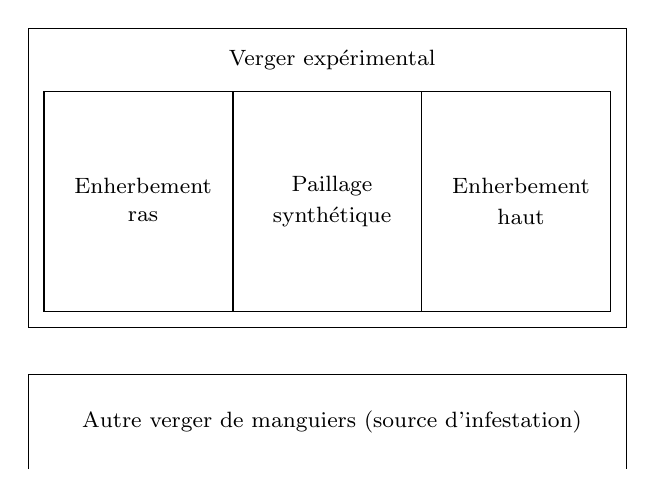
\begin{tikzpicture}[scale = 0.4]
  \draw (0,5) rectangle (18, 12);
  \draw (6, 5) -- (6, 12);
  \draw (12, 5) -- (12, 12);
  \draw (-0.5, 0) -- (-0.5, 3) ;
  \draw (-0.5, 3) -- (18.5, 3) ;
  \draw (18.5, 3) -- (18.5, 0);
  \draw (9, 1.5) node{\text{ \footnotesize Autre verger de manguiers (source d'infestation)}};
  \draw (9, 9) node{\text{ \footnotesize Paillage}};
  \draw (9, 8) node{\text{ \footnotesize synthétique}};
  \draw (3, 9) node{\text{ \footnotesize Enherbement}};
  \draw (3, 8) node{\text{ \footnotesize ras}};
  \draw (15, 9) node{\text{ \footnotesize Enherbement}};
  \draw (15, 8) node{\text{ \footnotesize haut}};
  \draw (-0.5, 4.5) rectangle (18.5, 14);
  \draw (9, 13) node{\text{ \footnotesize Verger expérimental }};
 \end{tikzpicture}
 \caption{Schéma de l'expérimentation menée. Le verger sur lequel ont été testées les trois modalités de couvertures du sol était situé à côté d'un autre verger, qui servait de source d'infestation. Cela fut fait pour garantir la présence de cécidomyies dans le verger expérimental.}
 \label{fig:exp}
\end{figure}

Sur ces deux vergers expérimentaux, deux types d'observations furent effectués entre juin et octobre 2017. 
Le premier porte sur les inflorescences. 
Huit unités de croissance furent sélectionnées sur chacun des vingt-cinq arbres tirés aléatoirement. 
Et c'est ainsi qu'entre le 26 juin et le 3 octobre 2017 furent notés les dates de débourrements des inflorescences présentes sur les deux cents unités de croissance suivies.
À partir du 6 septembre furent aussi notés les dates de morts des inflorescences. 
Les données de ce relevé seront rassemblées en un jeu de données que l'on nommera \emph{dataset 1}.

La seconde catégorie d'observations porte sur la capture des larves de cécidomyies.
Dans chacune des trois sous-parcelles, dix arbres furent sélectionnés. 
Sous chacun de ces arbres furent placés deux pièges en dessous des inflorescences présentes.
Les pièges sont des bidons plastiques carrés de douze centimètres de côté.
(À noter que les pièges furent déplacés au cours du temps pour qu'ils soient en-dessous du maximum d'inflorescences possibles.)
Et c'est ainsi qu'entre le 18 juillet et le 6 octobre 2017 furent notés le nombre de larves piégées, le nombre d'inflorescences vivantes au-dessus du piège et le nombre d'inflorescences vivantes dans l'arbre.
Les données de ce relevé seront rassemblées en un jeu de données que l'on nommera \emph{dataset 2}.

\section{Données}

Après mise en forme des données\footnote{Tous les scripts utilisés sont disponibles à l'adresse \url{https://github.com/bastienreyne/cecidomyie}}, on peut extraire les dynamiques qui nous intéressent.
Il faut cependant noter que les deux jeux de données n'ont pas la même échelle.
On choisira de tout mettre à l'échelle de la sous-parcelle.

\subsection{Inflorescences vivantes}

On peut avoir les dynamiques d'inflorescences vivantes grâce aux deux jeux de données.
Pour le \emph{dataset 2}, c'est facile. 
On possède le nombre d'inflorescences vivantes dans les arbres suivis aux différentes dates; il suffit alors de mettre à l'échelle comme suit :
\[
I_{t}^{2} = \frac{N}{n}\sum_{j=1}^{n} I^{2}_{j, t},
\]
avec $N$ représentant le nombre d'arbre dans la sous-parcelle, $n$ le nombre d'arbre suivis et $I^{2}_{j, t}$ le nombre d'inflorescences sur l'arbre $j$ à la date $t$.


Pour le \emph{dataset 1}, il faut récupérer le nombre de débourrements journalier $B_t$ et le nombre de morts journalier $D_t$; et le nombre d'inflorescences vivantes au jour $t$ s'écrit alors
\[
I_t^1 = \alpha\left( \sum_{j=1}^{t} B_j - \sum_{j=1}^{t} D_j \right),
\]
où $\alpha$ représente le coefficient de mise à l'échelle.
Il faut cependant apporter une correction cette dynamique.
En effet, l'observation des inflorescences mortes n'a été faite qu'à partir du 6 septembre.
De ce fait, sur ce jeu de données la distinction entre inflorescences vivantes et mortes n'est possible qu'à partir du 6 septembre.
Il en résulte un écart non-négligeable entre le 5 et le 6 septembre (voir figure~\ref{fig:inflos}).
Cet écart correspond au nombre de mort qu'il y a eu avant le 6 septembre, qu'il faut donc répartir sur la période concernée.
N'ayant aucune indication de comment la répartir, on utilisera la dynamique d'inflorescences vivantes du \emph{dataset 2} afin que la dynamique du \emph{dataset 1} y ressemble le plus possible --- et on en profitera au passage pour estimer le coefficient de mise à l'échelle $\alpha$.
Plus précisément, on attribuera un poids (à calibrer numériquement) pour tous les jours entre le jour 1 et le 5 septembre, et le nombre de morts chaque jour sera donné par la formule
\[
D_{t}^{c} = \frac{p_t\times m}{\sum_{j}p_j},
\]
où $D_{t}^{c}$ désigne le nombre de mort à la date $t$, $m$ le nombre de mort total déterminé par la différence d'inflorescences entre le 5 et 6 septembre et $p_t$ le poids assigné au jour $t$. 
Les poids $p_t$ et le coefficient de mise à l'échelle $\alpha$ seront déterminés numériquement afin de résoudre le problème
\[
\arg\max_{\alpha, p_t} \sum_{t}\left|I^{2}_{t} - I_{t}^{1, c}\right|, 
\]
où $I_{t}^{1, c}$ représente les inflorescences vivantes du \emph{dataset 1} mises à l'échelle et corrigées ; cette dynamique est determinée par la formule
\[
I_{t}^{1, c} = \begin{cases}
                I_t^1 - D_t^{c} & \text{si } t \leq 6 \text{ septembre},\\
                I_t^1 & \text{sinon}.
               \end{cases}
\]
Les différentes dynamiques d'inflorescences sont visibles sur la figure~\ref{fig:inflos}.
On remarque des dynamiques très différentes pour la modalité «enherbement haut», et ce même après correction de la dynamique issue du premier \emph{dataset}.
On peut expliquer ce phénomène par la grande variabilité de la phénologie chez le manguier ; ainsi un échantillonage peut produire des dynamiques très différentes.
Les deux autres modalités ont en revanche des dynamiques similaires (après correction).
\begin{figure}[ht]
\centering
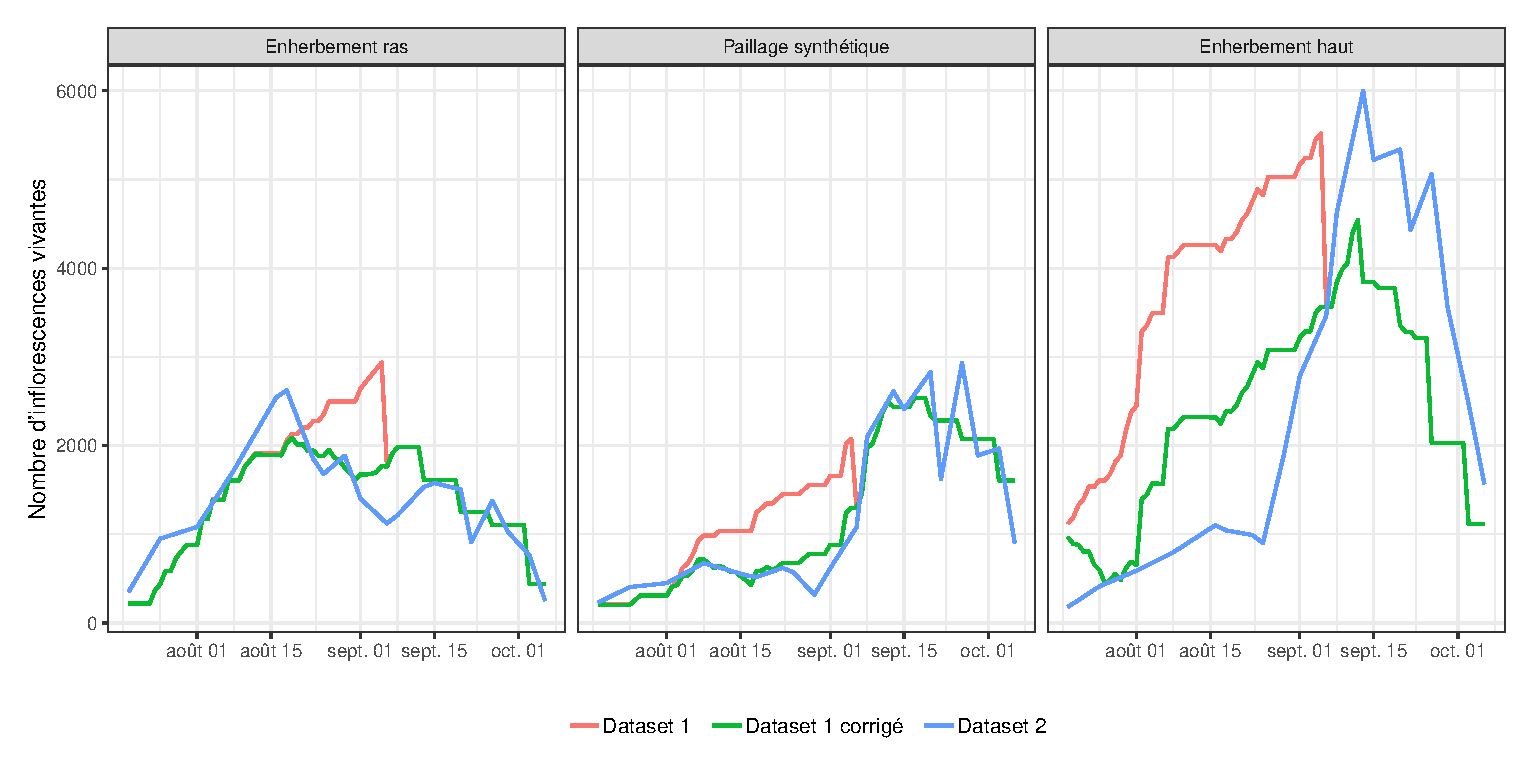
\epsfig{file = r/inflos_vivantes.eps, scale = 0.59}
\caption{Comparaison des différentes dynamiques d'inflorescences vivantes du verger n\textdegree1 en fonction du \emph{dataset} utilisé. Si après correction les dynamiques des deux \emph{datasets} sont similaires pour les deux premières modalités, la modalité «enherbement haut» présente des différences significatives entre les deux dynamiques. Cela peut s'expliquer par un échantillonage différent d'un phénomène présentant une grande variabilité.}
\label{fig:inflos}
\end{figure}

\subsection{Larves}

Le \emph{dataset 2} permet aussi de récupérer la dynamique de larves, à partir des larves piégées.
En effet, on connait le nombre de larves par piège, le nombre d'inflorescences vivantes situées au-dessus des pièges et le nombre d'inflorescences vivantes dans les arbres suivis.
De là, on peut estimer le nombre de larves qui s'éjecte des inflorescences à l'échelle d'un arbre, puis à l'échelle de la sous-parcelle.
Les différentes dynamiques de larves sont visibles sur la figure~\ref{fig:larves}.
Les relevés des pièges n'étant pas quotidien, le nombre de larves piégées a été reparti uniformément entre deux relevés, ce qui explique les «plateaux» visibles sur le graphique.
\begin{figure}[ht]
\centering
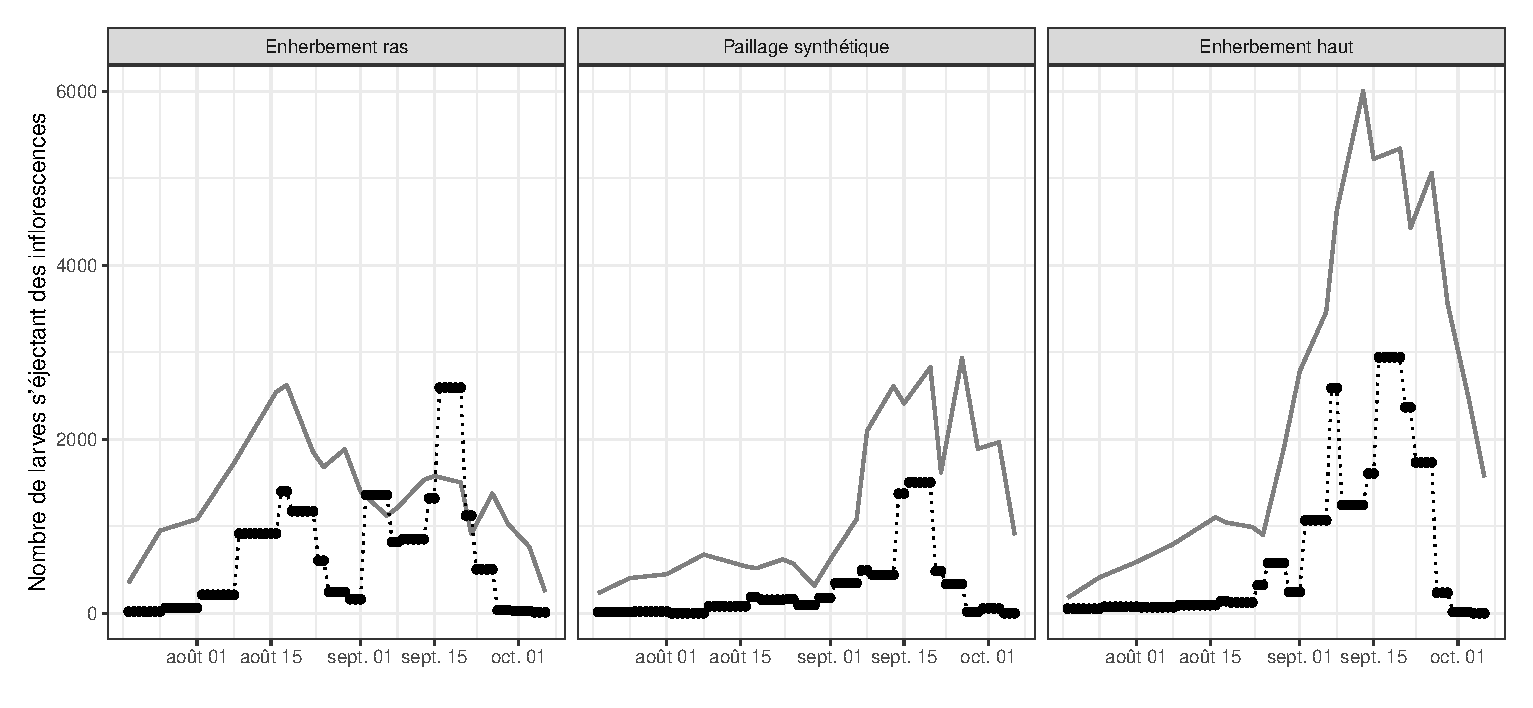
\epsfig{file = r/larves.eps, scale = 0.59}
\caption{Dynamiques de larves s'éjectant des manguiers chaque jour dans le verger n\textdegree1 pour chacune des trois sous-parcelles. En gris sont visibles les dynamiques d'inflorescences vivantes.}
\label{fig:larves}
\end{figure}


